\documentclass[11pt,a4paper]{article}

%==============================================================================%

\usepackage{a4wide}
\usepackage{amsmath,amssymb}
\usepackage[utf8]{inputenc}
\usepackage{float}
\usepackage{graphicx}
\usepackage{listings}
\usepackage{multicol}
\usepackage{tikz}

\usetikzlibrary{arrows}

%==============================================================================%

\newcommand{\assignmentnumber}{3}

\newcommand{\modulus}[1]{\lvert#1\rvert}
\newcommand{\conjugate}[1]{\bar{#1}}
\newcommand{\degree}{^{\circ}}
\newcommand{\limit}[2]{\lim_{#1 \rightarrow #2}}

\newcommand{\figref}[1]{fig. \ref{fig:#1}}
\newcommand{\eqnref}[1]{(\ref{eqn:#1})}

\DeclareMathOperator{\re}{Re}
\DeclareMathOperator{\im}{Im}

\renewcommand\thesection{\assignmentnumber.\arabic{section}}
\renewcommand\thesubsection{\alph{subsection})}

%==============================================================================%

\title{MatIntro Pointopgave \assignmentnumber}
\author
{
    Casper B. Hansen\\
    University of Copenhagen\\
    {\tt fvx507@alumni.ku.dk}
}
\date{\today}

%==============================================================================%

\begin{document}

% \maketitle


% 3.1
\section
{
    \mdseries
    Lad $f(x) = \frac{1}{x} - \frac{\cos x}{\sin x}$ for alle $x \in
    \mathbb{R}$ med $x \neq n\pi, n \in \mathbb{Z}$.
}
Til følgende opgaver defineres følgende erklæres følgende udsagn i Maple.
\begin{lstlisting}
    f := x -> (1/x) - cos(x)/sin(x)
\end{lstlisting}

% 3.1 (a)
\subsection
{
    \mdseries
    Find grænseværdierne $\limit{x}{0+} f(x)$, $\limit{x}{\pi-} f(x)$ først
    med og dernæst uden Maple.
}
I Maple skriver vi følgende
\begin{lstlisting}
    limit(f(x), x=0, right);
    limit(f(x), x=pi, left);
\end{lstlisting}
og får resultaterne $0$ hhv. $\frac{1}{\pi} - \frac{\cos \pi}{\sin \pi}$.

\begin{multicols}{2}
    Ved håndregning af $\limit{x}{0+} f(x)$ benytter vi reglen $\limit{x}{a}
    f(x) + g(x) = \limit{x}{a} f(x) + \limit{x}{a} g(x)$, og ser at
    førsteledet $\limit{x}{0+} \frac{1}{x} = \infty$ og at andetledet
    $\limit{x}{0+} \frac{\cos x}{\sin x} = \infty$.
    
    Vi har derfor, at $\limit{x}{0+} f(x) = \infty - \infty = 0$.
    
    \vfill{\ }\columnbreak

    På samme måde, ved håndregning af $\limit{x}{\pi-} f(x)$ har vi at
    $\limit{x}{\pi-} \frac{1}{x} = \frac{1}{\pi-}$ og at $\limit{x}{\pi-}
    \frac{\cos x}{\sin x} = ?$.

\end{multicols}

% 3.1 (b)
\subsection
{
    \mdseries
    Vis, at $f$ er strengt voksende i hvert interval $(n\pi,(n+1)\pi)$.
    Uligheden $\modulus{\sin x} < \modulus{x}$ for $x \neq 0$ kan benyttes
    uden bevis (den er vist i TLO side 240).
}
...

% 3.1 (c)
\subsection
{
    \mdseries
    Bevis, at ligningen $f(x) = 0$ ikke har nogen løsninger i $(0, \pi)$, og
    at den har præcis én løsning i $(\pi,2\pi)$. Benyt Maple til at finde en
    approksimering til denne løsning.
}
...


% 3.2
\section
{
    \mdseries
    En funktion $f : \mathbb{R} \rightarrow \mathbb{R}$ defineres ved
    \eqnref{3.2}
}
\begin{align}
    f(x) &=
    \begin{cases}
        \frac{1 - x^2}{(x -1)(x - 3)} &x \in (-\infty;1) \cup (3;\infty) \\
        x &x \in [1;3]
    \end{cases}
    \label{eqn:3.2}
\end{align}

I Maple har jeg erklæret funktionen, som følger
\begin{lstlisting}
c1 := x -> x < 1 or x > 3
c2 := x -> 1 <= x <= 3

f1 := x -> (1 - x^2) / ((x - 1)(x - 3))
f2 := x -> x

f  := x -> piecewise(c1(x), f1(x), c2(x), f2(x))
\end{lstlisting}

\begin{multicols}{2}
    % 3.2 (a)
    \subsection
    {
        \mdseries
        Lav i Maple et plot af et udsnit af grafen for $f$, der giver et
        retvisende og oplysende billede af funktionens overordnede opførsel.
    }

    \begin{figure}[H]
        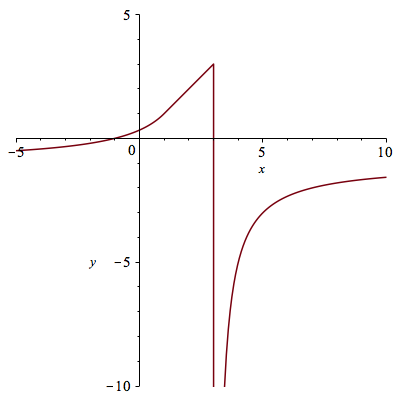
\includegraphics[scale=0.5]{figures/3-2a-1.png}
        \caption{Grafen for $f$ i intervallet $x,y \in [-5,10]$}
        \label{fig:3.2a-1}
    \end{figure}

    \vfill{\ }\columnbreak

    % 3.2 (b)
    \subsection
    {
        \mdseries
        Er $f$ differentiabel i $x=1$? Begrund dit svar uden brug af Maple.
    }
    ...

\end{multicols}


% 3.3 (iii)
\section
{
    (iii) \mdseries
    Betragt funktionen $f(x) = x(\ln(x + 1) - \ln x), x > 0$.
}

% 3.3 (iii) (a)
\subsection
{
    \mdseries
    Tegn grafen for $0 < x \leq 100$ og gæt på $\limit{x}{\infty} f(x)$ ud
    fra denne.
}
\begin{multicols}{2}
    Funktionen defineres og plottes i Maple som
\begin{lstlisting}
f := x -> x (ln(x + 1) - ln(x))

plot(f(x), x=0..100)
\end{lstlisting}
    
    Mit umiddelbare gæt er, at funktionen er asymptote med $y = 1$, og derfor
    at $\limit{x}{\infty} f(x) = 1$.

    \vfill{\ }\columnbreak

    \begin{figure}[H]
        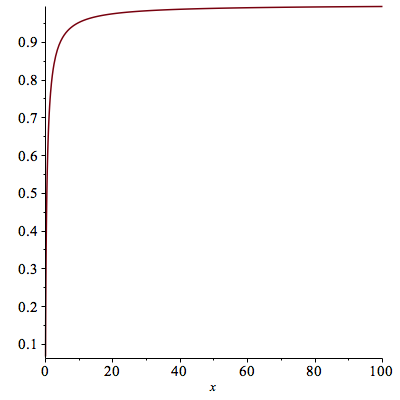
\includegraphics[scale=0.5]{figures/3-3(iii)a-1.png}
        \caption{Grafen for $f$ i intervallet $x \in [0,100]$}
        \label{fig:3.3(iii)a-1}
    \end{figure}

\end{multicols}


% 3.3 (iii) (b)
\subsection
{
    \mdseries
    Beregn i Maple $f(10^n)$ for $n = 1, \dots, 10$ (brug f. eks. værdien 20
    af Digits=antal decimaler). Gæt igen på $\limit{x}{\infty} f(x)$ ud fra
    disse tal.
}
\begin{multicols}{2}
    
    I Maple angiver jeg
\begin{lstlisting}
Digits := 22

evalf(f(10^1))
evalf(f(10^2))
evalf(f(10^3))
evalf(f(10^4))
evalf(f(10^5))
evalf(f(10^6))
evalf(f(10^7))
evalf(f(10^8))
evalf(f(10^9))
evalf(f(10^10))
\end{lstlisting}

    \vfill{\ }\columnbreak

    Og får følgende resultater;
    \begin{align}
        f(10^1)     &= 0.953100179804324860044 \\
        f(10^2)     &= 0.9950330853168082848 \\
        f(10^3)     &= 0.999500333083533167 \\
        f(10^4)     &= 0.99995000333308335 \\
        f(10^5)     &= 0.999995000033333 \\
        f(10^6)     &= 0.99999950000033 \\
        f(10^7)     &= 0.99999995000000 \\
        f(10^8)     &= 0.99999999500000 \\
        f(10^9)     &= 0.99999999950000 \\
        f(10^{10})  &= 0.99999999995000
    \end{align}

\end{multicols}

Hvilket stemmer meget godt overens med mit første gæt, og mit er derfor
uændret, ud fra disse resultater.

% 3.3 (iii) (c)
\subsection
{
    \mdseries
    Bestem $\limit{x}{\infty} f(x)$ uden brug af Maple. Kommenter resultaterne
    fra (a) og (b).
}
\begin{align}
    \limit{x}{\infty} f(x)
    &= \limit{x}{\infty} x (\ln(x + 1) - \ln(x)) \\
    &= \limit{x}{\infty} x
       \cdot
       \left(
           \limit{x}{\infty} \ln(x + 1) - \limit{x}{\infty} \ln(x)
       \right) \\
    &= \limit{x}{\infty} x
       \cdot
       \left(
           \limit{x}{\infty} \ln(x + 1) - \limit{x}{\infty} \ln(x)
       \right)
\end{align}

\end{document}
